\documentclass[t]{beamer}


	% Appearance:
	
	\usetheme{KTHprofile}
	\usefonttheme[onlylarge]{structurebold}
	
	% Standard packages
	
	\usepackage[english]{babel}
	%\usepackage[latin1]{inputenc}
	%\usepackage[utf8]
	\usepackage{times}
	\usepackage[T1]{fontenc}
	\usepackage{lipsum}
	
	% Author, Title, etc.
	
	%\title{}
	
	\title
	{DT2119 Speech and Speaker Recognition Lab 2
	}
	
	%\author{}
	
	\author[Zifan, Lingxi]
	{
	Zijian Fan, Lingxi Xiong
	}
	
	\institute{}
	
	%\institute[KTH Royal Institute of Technology]
	%{\inst{1} KTH Royal Institute of Technology, Sweden\and
	%\vskip-4mm
	%\inst{2} KTH Royal Institute of Technology, Sweden
	%}
	
	\date{}
	\date{\today}
	
	
	\begin{document}
	
\begin{frame}
	\titlepage
\end{frame}
	
\begin{frame}
	\frametitle{5.1 Gaussian emission probabilities}
	\begin{figure}
\centering
		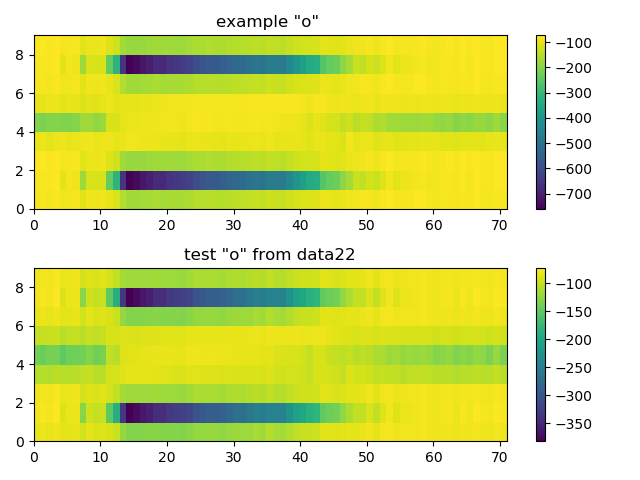
\includegraphics[width=0.65\textwidth]{figures/51.png}
	\end{figure}
			
	\begin{itemize}
		\item  isolated['o'] = ['sil'] + prondict['o'] + ['sil']
	\end{itemize}
\end{frame}
	
\begin{frame}
	\frametitle{5.2 Forward Algorithm}
	\begin{itemize}
		\item Maximum likelihood accuracy
		
trained on all speakers: 43/44

trained on one speaker: 34/44\\


		\item Viterbi algorithm accuracy

trained on all speakers: 44/44

trained on one speaker: 34/44 (same mistakes as ML)


\item Computational complexity

Viterbi scoring: \mathcal{O}(n)

Forward scoring: \mathcal{O}(n^2)

	\end{itemize}
\end{frame}
	

\begin{frame}
	\frametitle{5.3 Viterbi Approximation}
	\begin{figure}
\centering
		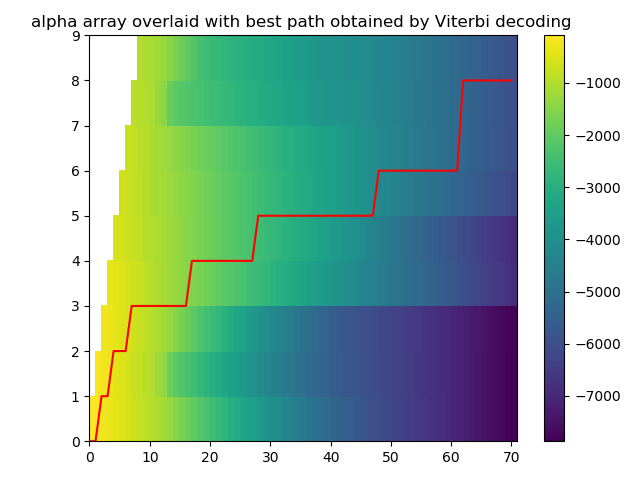
\includegraphics[width=0.55\textwidth]{figures/53.png}
	\end{figure}

	\begin{itemize}
		\item $\alpha_n(j) = P(x_0, ..., x_n, z_n =s_j \mid \theta)$
		\item $log V_n(j) = max^{M-1}_{i=0}(log V_{n-1}(i) + log a_{ij}) + log \phi_j(x_n)$
		\item $B_n(j) = argmax_{i=0}^{M-1}(log V_{n-1}(i) + log a_{ij})$
		

	\end{itemize}

	
\end{frame}
	
\begin{frame}
	\frametitle{5.4 Backward Algorithm}
	\begin{figure}
		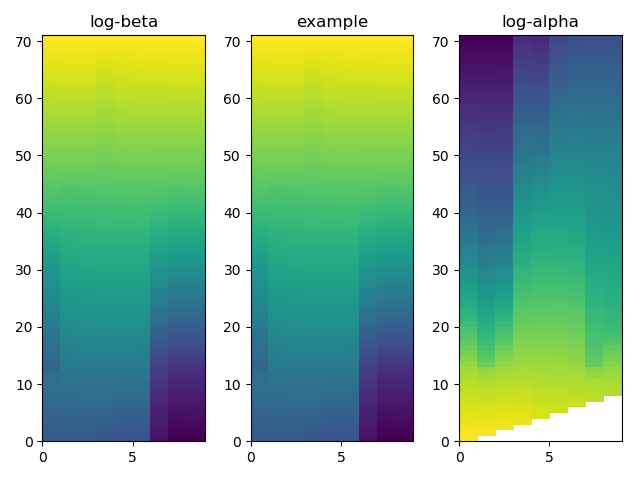
\includegraphics[width=0.6\textwidth]{figures/54.png}
	\end{figure}
 
\begin{itemize}
\item $\beta_n(i) = P(x_{n+1}, ..., x_{N-1} \mid z_n = s_i, \theta)$
\end{itemize}

\end{frame}
	
\begin{frame}
	\frametitle{6.1 State posterior(Gamma) probabilities}
	\begin{itemize}
		\item HMM posteriors: $\gamma_n(i) = P(z_n = s_i \mid X, \theta)$
		
		For each time step the state posteriors sum to 1 (in linear domain).\\

		Summing along the time axis: 1.35, 2.10, 3.56, 9.74, 10.12, 20.53, 13.00, 1.21, 9.40\\
		
		Summing over both states and time steps = length of the observation(71)

	\end{itemize}

\end{frame}
	
\begin{frame}
\frametitle{6.1 State posterior(Gamma) probabilities}
	\begin{figure}
		\centering
		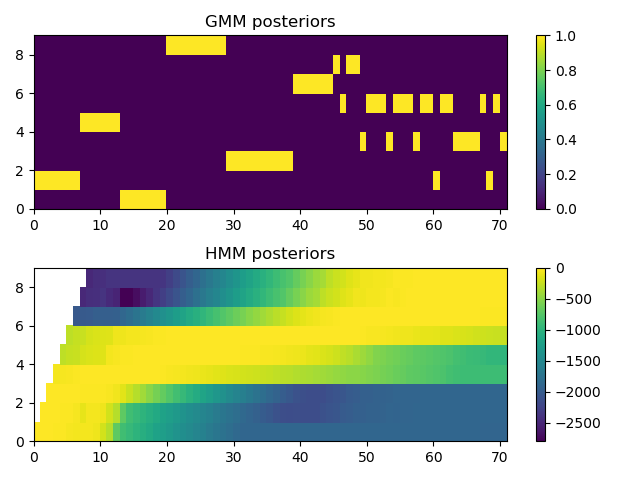
\includegraphics[width=0.65\textwidth]{figures/61.png}
	\end{figure}
	\begin{itemize}
		\item HMM posteriors: $\gamma_n(i) = P(z_n = s_i \mid X, \theta)$
		\item GMM posteriors: $\gamma_n^{GMM}(i) = P(z_n = s_i \mid x_n, \phi)$
	\end{itemize}


\end{frame}

\begin{frame}
	\frametitle{6.2 Retraining the emission probabilities distributions}
	\begin{figure}
\centering
		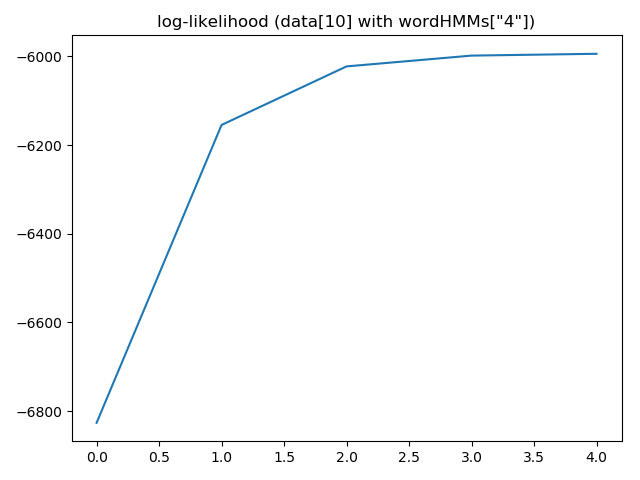
\includegraphics[width=0.48\textwidth]{figures/621.png}
		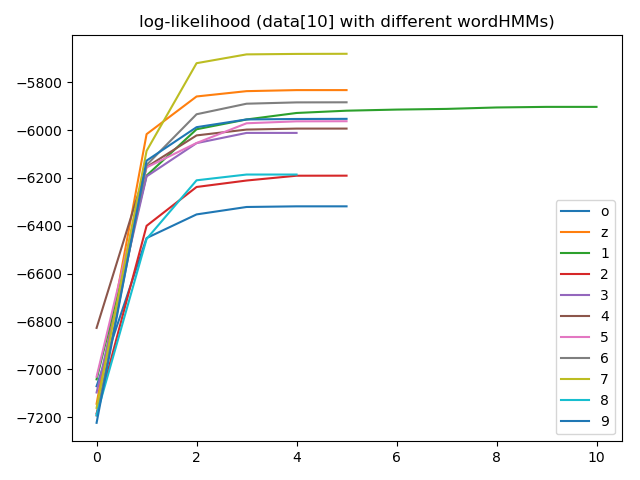
\includegraphics[width=0.48\textwidth]{figures/622.png}
	\end{figure}

\end{frame}

\begin{frame}
	\frametitle{Thank you for your Attention!}	
\end{frame}
	
\end{document}